\chapter{ОЗНАКОМЛЕНИЕ С УСТАНОВКОЙ DISYS МТ-SС-1}
Комплект <<Основы мехатроники>> модели DISYS МТ-SС-1 предназначен для изучения структуры, принципов построения и основной элементной базы автоматических линий и мехатронных систем.
Комплект представляет собой набор из четырех действующих моделей промышленных механизмов с пневматическими и электрическими приводами, а также устройств их ручного и программного управления.
Возможность комбинирования различного количества механизмов для совместной работы позволяет изучать в режиме <<от простого к сложному>> большое количество технологических операций и алгоритмов управления промышленными объектами. Комплект представлен на рисунке \ref{fig:all}.

Модели механизмов позволяют изучать:
\begin{itemize}
    \item Пневмоприводные системы и их элементную базу
    \item Электрические приводы
    \item Типы и области применения бесконтактных путевых выключателей
    \item Устройства ввода электрических сигналов
    \item Аппаратные и программные средства программируемых логических контроллеров
\end{itemize}


\begin{figure}[hb]
    \centering
    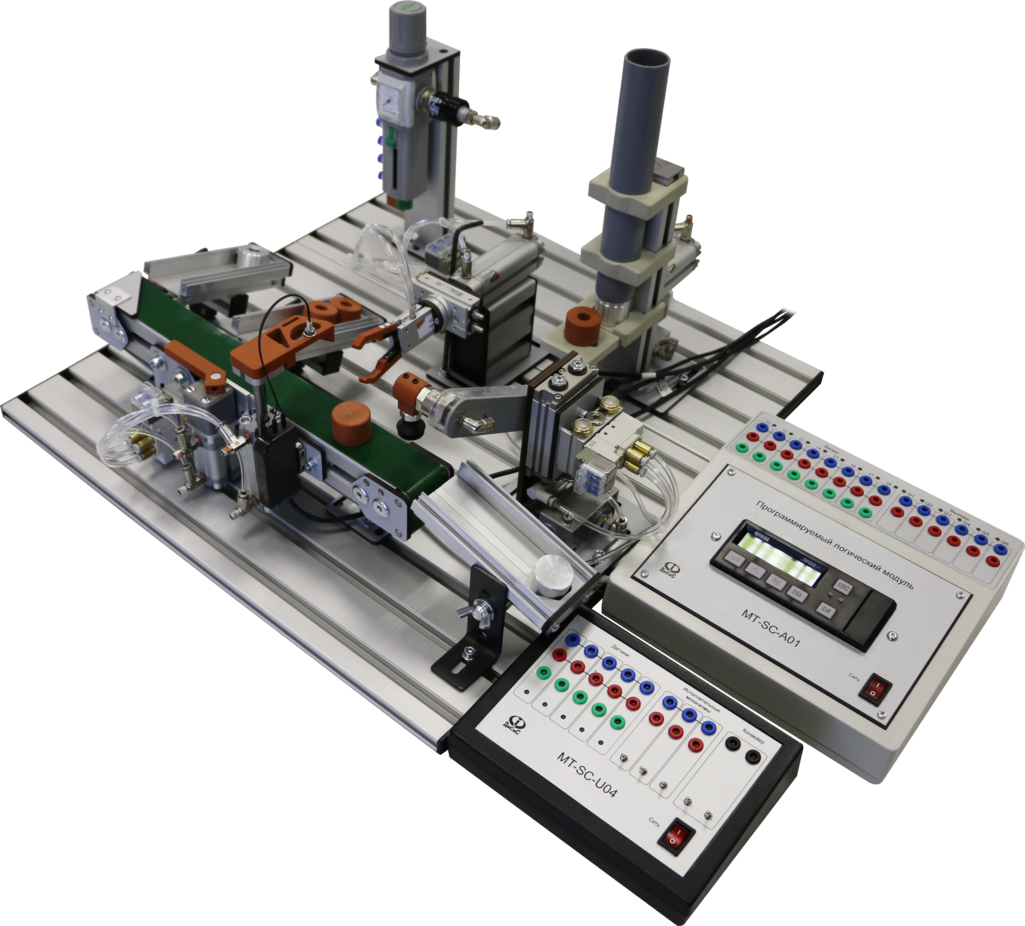
\includegraphics[scale=0.30]{fig/DISYS.png}
    \caption{Комплект <<Основы мехатроники>> модели DISYS МТ-SС-1>>}
    \label{fig:all}
\end{figure}

\section{Комплектность}
\begin{itemize}
    \item Гравитационный магазин
    \item Пневматический перекладчик
    \item Пневматический манипулятор
    \item Ленточный конвейер
    \begin{itemize}
        \item Оптический датчик с разнесенной оптикой (1шт.)
        \item Оптоволоконный датчик (1шт.)
        \item Индуктивный датчик (1шт.)
    \end{itemize}
    \item Информационная платформа
    \begin{itemize}
        \item Оптоволоконный датчик (не менее 2 шт.)
        \item Индуктивный датчик
    \end{itemize}
    \item Приемный лоток (не менее 4 шт.)
    \item Блок подготовки воздуха
    \item Герконовый датчик положения (не менее 13 шт.)
    \item Модуль ручного управления (не менее 4 шт.)
    \item Программируемый логический модуль (не менее 2 шт.)
    \item Монтажная плита (не менее 4 шт.) размер одной плиты не менее\\(ШхДхВ), мм 180х500х15
    \item Набор деталей; (пластиковый цилиндр, пластиковый стакан, металлический цилиндр и металлический стакан.3 шт.каждого типа)
\end{itemize}

\section{Технические характеристики}
\begin{table}[hb]
    \centering
    \begin{tabular}{m{108mm}|l}
    Масса, не более, кг              & 10          \\
    Габаритные размеры, мм (ШхГхВ)   & 600x600x350 \\
    Напряжение питания, В/Гц         & 220/50      \\
    Рабочее напряжение, пост. ток, В & 24          \\
    Рабочее давление, МПа            & 0,4
    \end{tabular}
\end{table}

Условия эксплуатации компонентов набора - в помещении при температурах от + 10 до + 35° С и относительной влажности воздуха до 80 \% при 25° С.